%
% File acl2020.tex
%
%% Based on the style files for ACL 2020, which were
%% Based on the style files for ACL 2018, NAACL 2018/19, which were
%% Based on the style files for ACL-2015, with some improvements
%%  taken from the NAACL-2016 style
%% Based on the style files for ACL-2014, which were, in turn,
%% based on ACL-2013, ACL-2012, ACL-2011, ACL-2010, ACL-IJCNLP-2009,
%% EACL-2009, IJCNLP-2008...
%% Based on the style files for EACL 2006 by 
%%e.agirre@ehu.es or Sergi.Balari@uab.es
%% and that of ACL 08 by Joakim Nivre and Noah Smith

\documentclass[11pt,a4paper]{article}
\usepackage[hyperref]{acl2020}
\usepackage{times}
\usepackage{latexsym}
\usepackage{graphicx}
\usepackage{qtree}
\renewcommand{\UrlFont}{\ttfamily\small}

% This is not strictly necessary, and may be commented out,
% but it will improve the layout of the manuscript,
% and will typically save some space.
\usepackage{microtype}

\aclfinalcopy % Uncomment this line for the final submission
%\def\aclpaperid{***} %  Enter the acl Paper ID here

%\setlength\titlebox{5cm}
% You can expand the titlebox if you need extra space
% to show all the authors. Please do not make the titlebox
% smaller than 5cm (the original size); we will check this
% in the camera-ready version and ask you to change it back.

\newcommand\BibTeX{B\textsc{ib}\TeX}

\title{Applying the Cascaded Finite State Grammar Induction Model to Trading Card Game Corpora}

\author{Kristian Mischke, Min Chon, Emily Sullivan, and Nathenael Dereb \\
  Department of Computer Science \\
  The University of Baltimore Maryland County \\
  Baltimore, MD 21250 \\
  \texttt{\{mischke1,minc1,emilys2,ndereb1\}@umbc.edu} \\}

\date{}

\begin{document}
\maketitle
\begin{abstract}
The goal of this project is to explore the effectiveness of an unsupervised Grammar Induction algorithm—specifically the Cascaded Finite State Model—by comparing its results on English natural language data to rules-text found on cards from the popular Trading Card Games: \emph{Magic: the Gathering}, \emph{Yu-Gi-Oh!}, \emph{Hearthstone}, and \emph{Keyforge}. Because this language is between an explicitly well-defined syntax like that of mathematical notation and natural languages (which contain ambiguity), we should expect better results than in the original paper. The language model perplexity reports that the model performance on TCG copra performs better than the Treebank-3 dataset.

\end{abstract}

\section{Introduction}
Grammar Induction is an algorithm that learns the grammar of a language by observing a set of data which is known to be valid under that language. Very little human input is required to build a model from grammar induction because it can be an unsupervised algorithm, which enables using large inputs from other sources. Grammar induction is also useful in pattern extraction given a large set of data; we can find patterns in text and establish a solid foundation for creating or validating new texts which use the same grammar. One way to approach grammar induction is the use of context-free grammars, a set of rules to define all possible values in a set of data. Context-free grammars help to organize what we consider significant in our data and create an outline of a generic statement, which may potentially assist in identifying or constructing new statements which fit into the grammar of the original set of data.

\emph{Magic: the Gathering} (MTG) and \emph{Yu-Gi-Oh!} are popular Trading Card Games (TCGs). TCGs are most commonly played without the need for a board or additional pieces. (with the exception of specific cards which may use the following: dice, coinflips, little tokens as counters, etc.) All that is needed to play a basic game is that both players have a valid deck of cards, an understanding of the overall rules of the game, and time. What sets TCGs apart from other games is that each card has its own unique set of rules which gives the player some advantage towards winning the game. Figure~\ref{mtg-card-layout} shows the layout of an MTG card, but all the TCGs we are concerned with have the same basic layout. Every card has a name at the top, and a body of text deemed the “rules-text”. These rules tend to follow a specific syntax regarding attack damage, statistical modifications, timing (e.g. end of turn), targets (e.g. creature/player), and other aspects of the game. The rule book of a TCG determines the base set of rules that outline how players take their turn and how they may take actions, but the cards’ individual rules-text augments the book rules, making the game more dynamic.
\begin{figure}[h]
	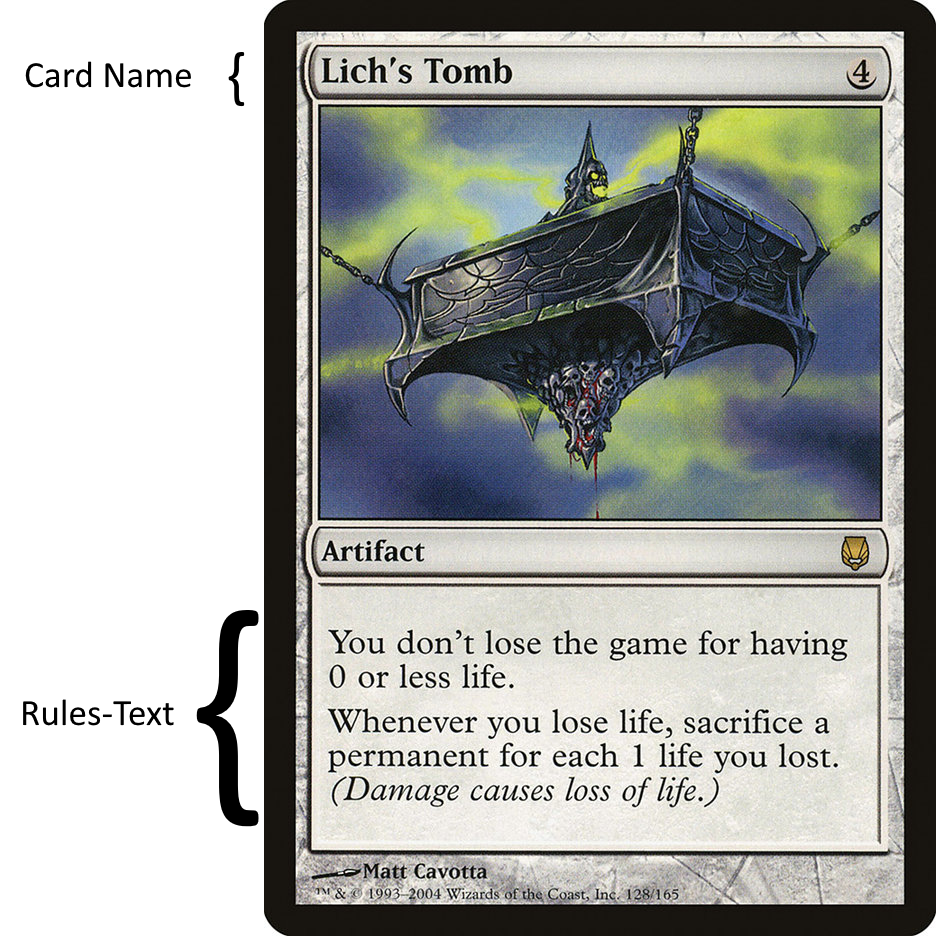
\includegraphics[width=\linewidth]{LichsTombMTGCardAnnotation.png}
	\caption{\label{mtg-card-layout} MTG card name and rules-text }
\end{figure}
For example, in MTG, Rule 704.5a states that “If at any time a player has 0 or less life, he or she loses the game.”\footnote{\url{https://media.wizards.com/2020/downloads/MagicCompRules\%2020201120.pdf}}. But if a player has the card \emph{Lich’s Tomb}, whose rules-text states “You don't lose the game for having 0 or less life. Whenever you lose life, sacrifice a permanent for each 1 life you lost.” then the book-rules are overridden for that player.

Choosing TCG cards for our analysis of grammar induction is ideal because most card games have a large number of samples for us to use when training our model. For example, MTG, the first TCG, currently has over 20,000 cards, and similar games like \emph{Yu-Gi-Oh!} have just under 5000 cards. Thus, we have enough data from the rules-text section of the cards, which we are most concerned about within our analysis. We often consider training a Grammar Induction model on unstructured data like human language. Some of the challenges of this are the fact that human languages incorporate things like ambiguity and complex phrasal structures. The motivation behind this project is to see if a Controlled Natural Language like that of the rules-text from a TCG improves the results of the model. Since TCG rules-text uses human language, it will still have some of these challenges, but it is made for games with well-defined rules so it is refined in scope and lacks many if not all of the ambiguities of natural language. Because it is a Controlled Natural Language, we believe that while the amount of data is definitely less than an average natural language dataset, it is large enough to train with. So we can expect our model to be well versed with the syntax of TCGs and able to produce results coherent to this context.

\section{Related Work}
Prior efforts were made to create grammars from MTG rules-texts. Some attempts at writing grammars are made by hand and are based on existing sets of cards. These grammars likely won’t generalize to all the rules of the game, therefore it may invalidate some text even though a player would consider it valid. Magarena\footnote{\url{https://github.com/magarena/magarena/blob/master/grammar/mtg.peg}} is an example of a hand-made grammar using parsing expression grammar. As a result of being hand-made, many representations of events in MTG may be long and specific to the referenced set of cards. Magarena has a non-terminal token named “AbilityRestriction” which repeats the rule “activate this ability only...” across all of its generations. For example, the generations continue with texts such as “...if seven or more cards are in your graveyard” or “...if you have no cards in hand”, without regard to different variations of the text (e.g. “graveyard” could be replaced with “battlefield”, and “cards” with “sorceries”). Our implementation automatically processes existing cards’ rules-text to determine the probability of a sequence of word types. The drawback compared to a hand-made grammar is the lack of annotation such as part-of-speech or any human-readable non-terminal tokens named after aspects of the game.

Some other developments that utilize MTG cards’ rules-texts include THELEMA by \citet{patsantzis_2015}, a project that creates a graph from sequential data, such as a grammar from sentences in a language. THELEMA was initially trained using the Controlled Natural Language (CNL) found in MTG, which is the cards’ rules-text. The CNL is considered akin to natural English, as it can be spoken and is both easily readable and writable, accompanied by syntax specific to MTG. While the goal of THELEMA is to define an explicit grammar for MTG along with production rules, our goal is simply to determine if parsing techniques perform better on CNL such as MTG rules-text than on human languages such as English.

\section{Proposed Solution}
For this project we will be implementing the unsupervised grammar induction model by \citet{ponvert-etal-2011-simple}. The motivation for this model is to formulate grammar induction as smaller text chunking sub-problems. The algorithm uses Probabilistic Right Linear Grammars (PRLGs) to determine the most likely constituents in a given sentence. It then combines the constituents as a pseudo-word and cascades the task to the next level. This repeated chunk and combine approach can be used to construct a parse tree for a given input sentence. In their work they used forward-backward expectation and maximization likelihood estimation with additive smoothing to estimate the model parameters. They chose this Expectation Maximization (EM) method because it works the same for both PRLGs and HMMs (Hidden Markov Models)—a model they compared results with.

These finite automata models both operate on the same hidden states used for sequence chunking. The states are: $B$ (which specifies the beginning of a chunk), $I$ (which specifies an intermediate token belonging to a chunk), $O$ (a token not belonging to a chunk), and $STOP$ (a token used for punctuation and sentence boundaries). The valid state transitions are given in Figure~\ref{state-diagram}. For our purposes a chunk is defined as a $B$ state followed by any number of I states. Because the algorithm is concerned with finding chunks that have more than one token in them there is no transition specified for $B \rightarrow B$.

\begin{figure}[h]
	\begin{center}
	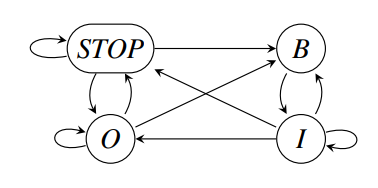
\includegraphics[width=2in]{figure1_state_diagram.png}
	\end{center}
	\caption{\label{state-diagram} State transition diagram used in \citet{ponvert-etal-2011-simple} }
\end{figure}

The cascading aspect of this algorithm can be formulated as follows, using an example from our data rephrasing the process given by \citet{ponvert-etal-2011-simple} for clarity over brevity:

\begin{enumerate}
	\item Start with raw tokenized text:
		
	\begin{center}\emph{destroy target land or nonblack creature . it ca n't be regenerated .}\end{center}	
	
	\item Apply the model using the Viterbi algorithm:	
	
	\begin{center}\emph{(destroy target land or nonblack) creature . it ca (n't be) regenerated .}\end{center}	
	
	\item Replace chunks with pseudowords:	
	
	\begin{center}\emph{\fbox{target} creature . it ca \fbox{be} regenerated .}\end{center}	
	
	\item Cascade by repeating steps 1--4 on the new sequence while chunks are still found in the sequence:
	
	\begin{center}\emph{(\fbox{target} creature) . (\fbox{it} regenerated) .}\end{center}
	
	\item Unravel to create a parse tree:	
	
	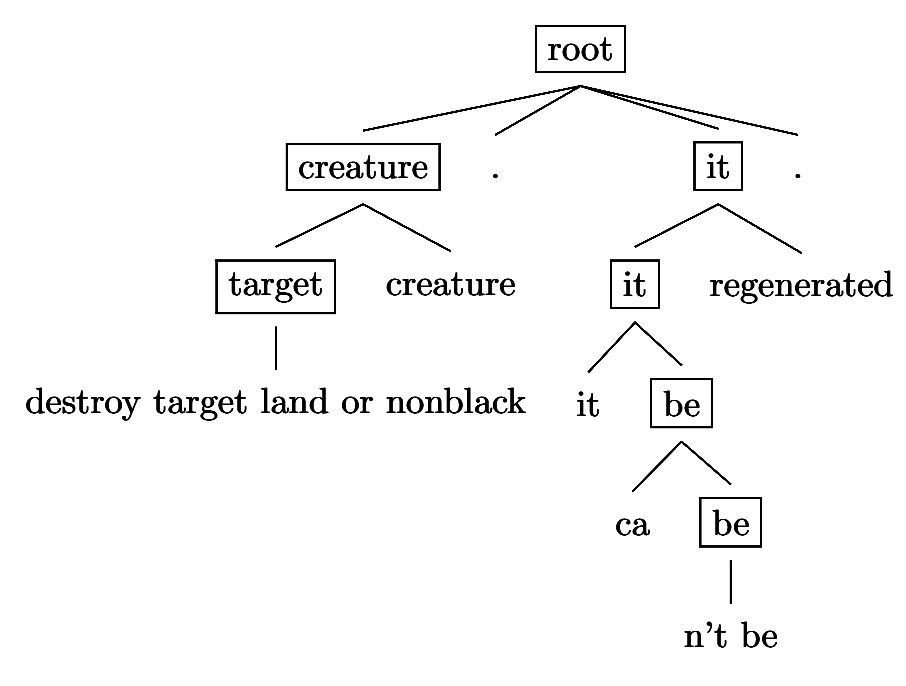
\includegraphics[width=\linewidth]{parse_tree_example.png}
\end{enumerate}

This process can be described as applying the chunking models in layers. After a given layer is chunked, the chunk is replaced with a pseudoword. \citet{ponvert-etal-2011-simple} found that using the token in the chunk with the highest corpus frequency was simple, but provided effective results. Additionally, the chunkers used at each level were initialized with the same parameters, tokens, and smoothing.

\section{Data}
We used data from four popular TCGs, namely: MTG, \emph{Yu-Gi-Oh!}, \emph{Hearthstone}, and \emph{Keyforge}. We accessed the MTG data from MTGJSON\footnote{\url{https://mtgjson.com/}} v5.0.1, an open source project that catalogues MTG cards. MTG has a total of 21,328 cards. We obtained the \emph{Yu-Gi-Oh!} Data from YGOPRODeck v7\footnote{\url{https://db.ygoprodeck.com/api/v7/cardinfo.php}} which contains 10,998 cards. \emph{Hearthstone} has 10,528 cards, and we used the \emph{Hearthstone} JSON API v1\footnote{\url{https://api.hearthstonejson.com/v1/66927/enUS/cards.json}} to obtain them. \emph{Keyforge} has 258 cards, and we accessed the data from a JSON repo on GitHub\footnote{\url{https://github.com/keyforg/keyforge-cards-json/blob/master/cards.json}}.

We used a 60-20-20 split for each dataset. Therefore the splits were as follows: MTG (12,792 train, and 4,266 dev \& test), \emph{Yu-Gi-Oh!} (6,598 train, 2,200 dev \& test), \emph{Hearthstone} (6,316 train, 2,106 dev \& test), and \emph{Keyforge} (214 train, 72 dev \& test). During training the evaluation sets were kept blind to the model.

\section{Evaluation and Testing}
Similar to \citet{ponvert-etal-2011-simple}, we will base our evaluation on identifying multi-word chunks of all constituent types and test our model on the Penn Treebank-3 dataset to ensure our model is correctly implemented and follows the results from the paper. Once we have verified this, we will evaluate the results we get for the TCG datasets. We will utilize PRLG, as our primary evaluation model and compare it against an HMM model as a benchmark. This will allow us to validate our results as information is lost due to the independence assumption characteristic of an HMM model. By comparing it against PRLG we should expect PRLG to perform better as referenced in Ponvert et al. Model performance is reported on the results from computing language model perplexity. 

To compute sentence perplexity we first computed the log marginal likelihood, $P(w_1,... w_n)$, using the Baum-Welch forward algorithm in log-space to account for underflow. 

\begin{center}
\small
$perplexity(w_1, ... w_n) = exp(\frac{-1}{n} P(w_1,... w_n))$
\normalsize
\end{center}

To compute corpus perplexity, we compute the log marginal likelihood of each sentence and propagate the probabilities to compute corpus perplexity. The probabilities of each sentence, $s_i$ is summed rather than multiplied because the probabilities are computed in log-space.

\begin{center}
$P(s_1, ..., s_n) = \sum_{i=1}^n P(s_i)$
\end{center}

$P(s_i)$ is the log marginal likelihood of a sentence, $s_i$

\begin{center}
$perplexity(corpus) = exp(\frac{-1}{N} P(s_1, ..., s_n))$
\end{center}

\section{Experimentation}
Our experimentation lies primarily within our model parameters. We tried a couple of different variations to try to understand more about the model. We were curious if the model could generalize if we trained it on more than one TCG, so we combined all the TCG datasets together as one option. Because it is common among TCGs to include a card’s name within its rules-text, we created a preprocessing option that replaces instances of a card’s name with a predefined token labelled \textless this\textgreater, as well as replacing numeric sequences with a \textless number\textgreater token. In turn we ran all models (including the combined model) with and without the token replacement parameter. This gave us a total of 10 models to train (MTG, \emph{Yu-Gi-Oh!}, \emph{Hearthstone}, \emph{Keyforge}, and the combined model, each with and without the parameter set).

Parameters we could have experimented more with but kept constant were: OOV (Out Of Vocabulary) Threshold = 1, and we always converted the text to lowercase before tokenizing. We chose to run the models using PRLGs because \citet{ponvert-etal-2011-simple} discovered it to have better results than the HMM (but this could have been another parameter). For the same reasons, we also opted to use the STOP state for phrasal boundary tokens. We used:

\begin{center}
. \quad , \quad ; \quad ! \quad ? \quad `
\end{center}

\section{Results and Analysis}

We evaluated the performance of our model by computing perplexity for all the TCG datasets as shown in Figures~\ref{models-perplexity-replace} and~\ref{models-perplexity-no-replace}. Results for the Penn Treebank-3 dataset is shown in Figure~\ref{treebank-3-comparison}. 

As discussed in the Limitations of Work section, we faced limitations when computing additive smoothing for the probabilities. In order to account for this and avoid overfitting we decided to set the model to converge when the perplexity values began to increase in the test set.  

\begin{figure}[h]
	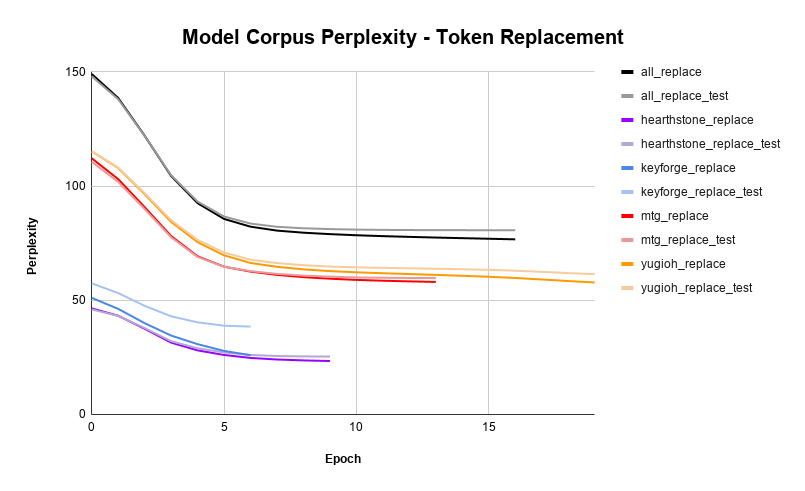
\includegraphics[width=\linewidth]{models_perplexity_replace.png}
	\caption{\label{models-perplexity-replace} TCG-Corpus Lang Model Perplexity with Token Replacements. }
\end{figure}

\begin{figure}[h]
	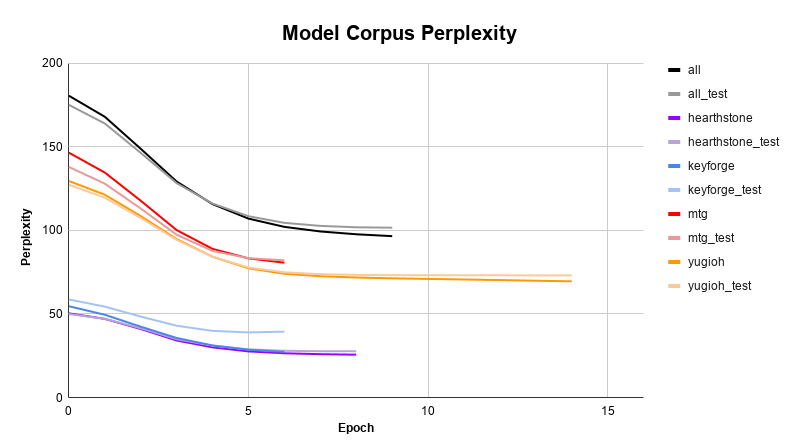
\includegraphics[width=\linewidth]{models_perplexity_no_replace.png}
	\caption{\label{models-perplexity-no-replace} TCG-Corpus Lang Model Perplexity }
\end{figure}

Figure~\ref{models-perplexity-replace} reports the results for the TCG datasets where token replacements for \textless this\textgreater and \textless number\textgreater  were replaced with instances of a card’s name and numeric sequences. We expected this model to perform better than the one reported in Figure~\ref{models-perplexity-no-replace} -- where there were no token replacements. For example, the test set for the MTG datasets for the model with token replacement, shown in Figure~\ref{models-perplexity-replace}, converged at 59.76. In Figure~\ref{models-perplexity-no-replace}, for the model with no token replacements converged at 82.07. Overall, the results report that the perplexity values in the model with token replacements are about 20 points lower than the model with no token replacements.

Figure~\ref{treebank-3-comparison} reports HMM and PRLG language model perplexity on the Penn Treebank-3 dataset. As expected and as referenced in Ponvert et al., the PRLG should perform better than the HMM model and our results show that the PRLG model performs better than the HMM model.

\begin{figure}[h]
	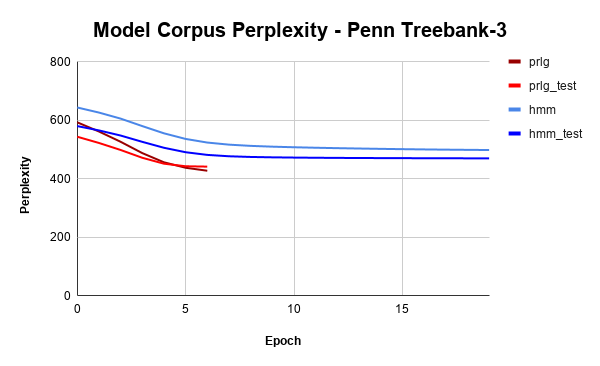
\includegraphics[width=\linewidth]{treebank_3_comparison.png}
	\caption{\label{treebank-3-comparison} Penn Treebank-3 Lang Model Perplexity HMM \& PRLG }
\end{figure}

The model with token replacement shows behaviour where it groups a verb followed by a determiner as a constituent. This is seen in the all\textunderscore replace dataset at epoch 8 and mtg\textunderscore replace dataset at epoch 16. Below are examples of such behaviours:

\Tree [. {enters the} {battlefield} ]
\hspace{0.05in}
\Tree [. {sacrifice a} {permanent} ]
\vspace{0.2in}
\Tree [. {discards a} {card} ]

This is undesirable because it goes against linguistic constituency structures. Although this could be explainable due to the fact that TCG rules often contain commands that start with verbs, a desirable constituency structure would be:

\Tree [. {enters} {the battlefield} ]
\hspace{0.05in}
\Tree [. {discards} {a card} ]

Despite these linguistic inconsistencies, the model reported better results according to the perplexity metric. We consider these results satisfactory.

\section{Limitations of Work}

The findings of this project have to be seen in light of some limitations. While completing our work, we found that time was one of the more extreme constraints. In the time we had left, we were unable to compute 10-fold cross-validation as we originally planned. Due to this issue, we instead ran our model without cross-validation, possibly giving us less accurate results. The second limitation regards lambda smoothing. We ran into issues with calculating it on probabilities and had to remove it completely from our results. In doing so we believe we are inhibiting our results slightly by declaring convergence earlier due to overfitting that occurs in later epochs. We also found, just as we assumed in the planning of our project to be potential blocks, that we could not calculate precision, recall, or F-scores like the original paper had done because the TCG dataset was unlabeled. This limits our findings by restricting us to less informative evaluation methods like perplexity. Also, while discussing calculating values, we ran into the issue of which data set to run the perplexity calculation on. The original reference paper did not clearly report their perplexity values or what data set they calculated on, so we had to use our best judgment. Since we decided to collect data from not only MTG cards but also other card games like \emph{Hearthstone} and \emph{Keyforge}, we speculated that the size of these two card populations could prove to be an issue which we found to be true as they had fewer cards available to use within our testing and the data ended up converging on fewer iterations. 

\section{Future Work}
Potential work that could be done in the short-term includes addressing any of our limitations (especially the ones due to lack of time). Additionally, more experimentation could be done to get a better idea of which parameters have the most impactful effect on the model. For example, we only compared training the model on the raw tokens vs ones with replaced \textless this\textgreater and \textless number\textgreater tokens--but never experimented with only one or the other. Further work should also go into determining why the constituencies do not match linguistic NP VP standards.

Longer-term work might include creating parse trees of the TCG rules by-hand so that accuracy, precision, recall, and F1 scores could be computed using the PARSEVAL method \citep{black-etal-1991-procedure}. Further work could also be done to compare other grammar induction techniques --perhaps state of the art methods using Neural Networks like the Compound PCFG model by \citet{kim-etal-2019-compound}--to see if they have the same benefits on Controlled Natural Language data like that of TCG rules-text.

\section{Conclusion}
This paper describes an approach to applying the cascaded finite state grammar induction model by \citet{ponvert-etal-2011-simple} to trading card game copra. We have explored how existing efforts on Grammar Induction perform better on CNL as found in TCGs. Specifically, in this paper we found that the model reported lower perplexity metrics than on the English Treebank-3 dataset \citep{treebank_3}. We found that a lower perplexity could be achieved by using a simple preprocessing technique to replace card names and numbers with special tokens. Despite the limitations of time and the compromise we made for lack of lambda smoothing, our results match our expectations. Finally, we expect these results would have similar trends using other Grammar Induction techniques.

\vspace{0.1in}
\noindent \textbf{Acknowledgements} Thanks to Dr. Ferraro for access to the Treebank-3 dataset and his input on our progress and hmm model implementation

\bibliography{anthology,acl2020}
\bibliographystyle{acl_natbib}

\end{document}
